\documentclass[aspectratio=169]{beamer}
\usepackage[utf8]{inputenc}
\usepackage{lmodern}
\usepackage[T1]{fontenc}
\usepackage{listings}
\usepackage{tikz}
\usetikzlibrary{arrows.meta, positioning, shapes.geometric, calc}

% Set path to find the theme
\makeatletter
\def\input@path{{../BeamerTemplate/theme/}}
\makeatother

\usetheme{CleanEasy}
\input{../BeamerTemplate/configs/configs}

% Listings configuration
\lstset{
    basicstyle=\ttfamily\footnotesize,
    keywordstyle=\color{blue},
    commentstyle=\color{gray},
    stringstyle=\color{red},
    showstringspaces=false,
    breaklines=true,
    frame=single,
    numbers=left,
    numberstyle=\tiny\color{gray}
}

\title{Sorting Algorithms}
\subtitle{Organize Data to Enable Efficient Access and Computation}
\author{Minseok Jeon}
\institute{DGIST}
\date{\today}

\begin{document}

\begin{frame}
  \titlepage
\end{frame}

\begin{frame}{Table of Contents}
  \tableofcontents
\end{frame}

\section{Introduction}

\begin{frame}{What is Sorting?}
  \textbf{Sorting}: Arranging data in a particular order (ascending/descending)

  \vspace{0.3cm}
  \textbf{Why Sorting Matters:}
  \begin{itemize}
    \item Foundation for search algorithms
    \item Database query optimization
    \item Data organization and visualization
    \item Algorithm efficiency (many algorithms require sorted data)
  \end{itemize}

  \vspace{0.3cm}
  \textbf{Classification:}
  \begin{itemize}
    \item \textbf{Comparison-based}: Compare elements pairwise
    \begin{itemize}
      \item Quick Sort, Merge Sort, Heap Sort
      \item Lower bound: $\Omega(n \log n)$
    \end{itemize}
    \item \textbf{Non-comparison}: Use element properties
    \begin{itemize}
      \item Counting Sort, Radix Sort, Bucket Sort
      \item Can achieve $O(n)$ time
    \end{itemize}
  \end{itemize}
\end{frame}

\begin{frame}{Key Properties of Sorting Algorithms}
  \textbf{Important Characteristics:}

  \vspace{0.3cm}
  \textbf{1. Time Complexity:}
  \begin{itemize}
    \item Best, Average, Worst case scenarios
  \end{itemize}

  \vspace{0.2cm}
  \textbf{2. Space Complexity:}
  \begin{itemize}
    \item In-place vs. requiring extra memory
  \end{itemize}

  \vspace{0.2cm}
  \textbf{3. Stability:}
  \begin{itemize}
    \item Preserves relative order of equal elements
  \end{itemize}

  \vspace{0.2cm}
  \textbf{4. Adaptability:}
  \begin{itemize}
    \item Performance on partially sorted data
  \end{itemize}

  \vspace{0.2cm}
  \textbf{5. Recursion:}
  \begin{itemize}
    \item Recursive vs. Iterative implementation
  \end{itemize}
\end{frame}

\section{Comparison Sorts: Quick/Merge/Heap}

\begin{frame}{Quick Sort: Overview}
  \textbf{Divide and Conquer Using Partitioning}

  \vspace{0.3cm}
  \textbf{Algorithm:}
  \begin{enumerate}
    \item Choose a pivot element
    \item Partition: elements $<$ pivot left, $>$ pivot right
    \item Recursively sort left and right partitions
  \end{enumerate}

  \vspace{0.3cm}
  \textbf{Characteristics:}
  \begin{itemize}
    \item \textbf{Time}: $O(n \log n)$ average, $O(n^2)$ worst
    \item \textbf{Space}: $O(\log n)$ for recursion stack
    \item \textbf{In-place}: Yes
    \item \textbf{Stable}: No
  \end{itemize}

  \vspace{0.3cm}
  \textbf{Advantages:}
  \begin{itemize}
    \item Fastest average-case performance
    \item Good cache locality
    \item In-place sorting
  \end{itemize}
\end{frame}

\begin{frame}[fragile]{Quick Sort: Implementation}
\begin{lstlisting}[language=Python, basicstyle=\ttfamily\tiny]
def quick_sort(arr, low, high):
    """Sort array using quick sort"""
    if low < high:
        # Partition and get pivot index
        pivot_idx = partition(arr, low, high)

        # Recursively sort left and right
        quick_sort(arr, low, pivot_idx - 1)
        quick_sort(arr, pivot_idx + 1, high)

def partition(arr, low, high):
    """Lomuto partition scheme"""
    pivot = arr[high]  # Choose last element as pivot
    i = low - 1  # Index of smaller element

    for j in range(low, high):
        if arr[j] <= pivot:
            i += 1
            arr[i], arr[j] = arr[j], arr[i]

    # Place pivot in correct position
    arr[i + 1], arr[high] = arr[high], arr[i + 1]
    return i + 1
\end{lstlisting}
\end{frame}

\begin{frame}{Quick Sort: Example}
  \textbf{Sorting: [7, 2, 1, 6, 8, 5, 3, 4]}

  \vspace{0.3cm}
  \textbf{Step 1:} Choose pivot = 4 (last element)

  \textbf{Step 2:} Partition
  \begin{center}
  Before: [7, 2, 1, 6, 8, 5, 3, 4]

  After: [2, 1, 3, 4, 8, 5, 7, 6]

  \vspace{0.2cm}
  Elements $< 4$ on left, $> 4$ on right
  \end{center}

  \vspace{0.3cm}
  \textbf{Step 3:} Recursively sort [2, 1, 3] and [8, 5, 7, 6]

  \vspace{0.2cm}
  \textbf{Final Result:} [1, 2, 3, 4, 5, 6, 7, 8]
\end{frame}

\begin{frame}{Merge Sort: Overview}
  \textbf{Divide and Conquer with Merging}

  \vspace{0.3cm}
  \textbf{Algorithm:}
  \begin{enumerate}
    \item Divide array into two halves
    \item Recursively sort each half
    \item Merge the two sorted halves
  \end{enumerate}

  \vspace{0.3cm}
  \textbf{Characteristics:}
  \begin{itemize}
    \item \textbf{Time}: $O(n \log n)$ always
    \item \textbf{Space}: $O(n)$ for auxiliary array
    \item \textbf{In-place}: No
    \item \textbf{Stable}: Yes
  \end{itemize}

  \vspace{0.3cm}
  \textbf{Advantages:}
  \begin{itemize}
    \item Guaranteed $O(n \log n)$ performance
    \item Stable sorting
    \item Good for external sorting (disk-based)
    \item Parallelizable
  \end{itemize}
\end{frame}

\begin{frame}[fragile]{Merge Sort: Implementation}
\begin{lstlisting}[language=Python, basicstyle=\ttfamily\tiny]
def merge_sort(arr):
    """Sort array using merge sort"""
    if len(arr) <= 1:
        return arr

    # Divide
    mid = len(arr) // 2
    left = merge_sort(arr[:mid])
    right = merge_sort(arr[mid:])

    # Conquer (merge)
    return merge(left, right)

def merge(left, right):
    """Merge two sorted arrays"""
    result = []
    i = j = 0

    # Merge while both have elements
    while i < len(left) and j < len(right):
        if left[i] <= right[j]:
            result.append(left[i])
            i += 1
        else:
            result.append(right[j])
            j += 1

    # Add remaining elements
    result.extend(left[i:])
    result.extend(right[j:])

    return result
\end{lstlisting}
\end{frame}

\begin{frame}{Merge Sort: Example}
  \textbf{Sorting: [38, 27, 43, 3, 9, 82, 10]}

  \vspace{0.3cm}
  \textbf{Divide Phase:}
  \begin{center}
  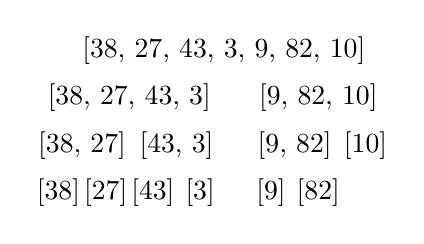
\begin{tikzpicture}[scale=0.6]
    \node at (0,0) {[38, 27, 43, 3, 9, 82, 10]};
    \node at (-2,-1) {[38, 27, 43, 3]};
    \node at (2,-1) {[9, 82, 10]};
    \node at (-3,-2) {[38, 27]};
    \node at (-1,-2) {[43, 3]};
    \node at (1.5,-2) {[9, 82]};
    \node at (3,-2) {[10]};
    \node at (-3.5,-3) {[38]};
    \node at (-2.5,-3) {[27]};
    \node at (-1.5,-3) {[43]};
    \node at (-0.5,-3) {[3]};
    \node at (1,-3) {[9]};
    \node at (2,-3) {[82]};
  \end{tikzpicture}
  \end{center}

  \vspace{0.3cm}
  \textbf{Merge Phase:}
  \begin{center}
  Merge pairs: [27, 38], [3, 43], [9, 82]

  Merge again: [3, 27, 38, 43], [9, 10, 82]

  Final merge: [3, 9, 10, 27, 38, 43, 82]
  \end{center}
\end{frame}

\begin{frame}{Heap Sort: Overview}
  \textbf{Build Max Heap, Repeatedly Extract Maximum}

  \vspace{0.3cm}
  \textbf{Algorithm:}
  \begin{enumerate}
    \item Build a max heap from input array
    \item Repeatedly extract maximum (root)
    \item Place extracted element at end of array
    \item Restore heap property
  \end{enumerate}

  \vspace{0.3cm}
  \textbf{Characteristics:}
  \begin{itemize}
    \item \textbf{Time}: $O(n \log n)$ always
    \item \textbf{Space}: $O(1)$
    \item \textbf{In-place}: Yes
    \item \textbf{Stable}: No
  \end{itemize}

  \vspace{0.3cm}
  \textbf{Advantages:}
  \begin{itemize}
    \item Guaranteed $O(n \log n)$ performance
    \item In-place sorting (no extra memory)
    \item No worst-case degradation
  \end{itemize}
\end{frame}

\begin{frame}[fragile]{Heap Sort: Implementation}
\begin{lstlisting}[language=Python, basicstyle=\ttfamily\tiny]
def heap_sort(arr):
    """Sort array using heap sort"""
    n = len(arr)

    # Build max heap
    for i in range(n // 2 - 1, -1, -1):
        heapify(arr, n, i)

    # Extract elements from heap
    for i in range(n - 1, 0, -1):
        # Move current root to end
        arr[0], arr[i] = arr[i], arr[0]

        # Heapify reduced heap
        heapify(arr, i, 0)

def heapify(arr, n, i):
    """Maintain max heap property"""
    largest = i
    left = 2 * i + 1
    right = 2 * i + 2

    # Check if left child is larger
    if left < n and arr[left] > arr[largest]:
        largest = left

    # Check if right child is larger
    if right < n and arr[right] > arr[largest]:
        largest = right

    # If largest is not root
    if largest != i:
        arr[i], arr[largest] = arr[largest], arr[i]
        heapify(arr, n, largest)
\end{lstlisting}
\end{frame}

\begin{frame}{Comparison of Quick/Merge/Heap}
  \begin{center}
  \begin{tabular}{|l|c|c|c|}
    \hline
    \textbf{Property} & \textbf{Quick Sort} & \textbf{Merge Sort} & \textbf{Heap Sort} \\
    \hline
    Best Time & $O(n \log n)$ & $O(n \log n)$ & $O(n \log n)$ \\
    \hline
    Average Time & $O(n \log n)$ & $O(n \log n)$ & $O(n \log n)$ \\
    \hline
    Worst Time & $O(n^2)$ & $O(n \log n)$ & $O(n \log n)$ \\
    \hline
    Space & $O(\log n)$ & $O(n)$ & $O(1)$ \\
    \hline
    Stable & No & Yes & No \\
    \hline
    In-place & Yes & No & Yes \\
    \hline
  \end{tabular}
  \end{center}

  \vspace{0.3cm}
  \textbf{When to Use:}
  \begin{itemize}
    \item \textbf{Quick Sort}: General purpose, fastest average case
    \item \textbf{Merge Sort}: Need stability or guaranteed performance
    \item \textbf{Heap Sort}: Limited memory, guaranteed performance
  \end{itemize}
\end{frame}

\section{Stability and In-Place Properties}

\begin{frame}{What is Stability?}
  \textbf{Stability}: Maintains relative order of equal elements

  \vspace{0.3cm}
  \textbf{Example:}
  \begin{center}
  Original: [(3, "a"), (1, "b"), (3, "c"), (2, "d")]

  \vspace{0.2cm}
  Sort by first element:

  \vspace{0.2cm}
  \textbf{Stable}: [(1, "b"), (2, "d"), (3, "a"), (3, "c")]

  {\color{blue} "a" before "c" (order preserved)}

  \vspace{0.2cm}
  \textbf{Unstable}: [(1, "b"), (2, "d"), (3, "c"), (3, "a")]

  {\color{red} "c" before "a" (order changed)}
  \end{center}
\end{frame}

\begin{frame}{Why Stability Matters}
  \textbf{Multi-level Sorting:}

  \vspace{0.3cm}
  \textbf{Example: Sort students by grade, then by name}

  \begin{enumerate}
    \item First sort by name (stable):
    \begin{itemize}
      \item [(Alice, 85), (Bob, 90), (Charlie, 85), (David, 90)]
    \end{itemize}

    \vspace{0.2cm}
    \item Then sort by grade (stable):
    \begin{itemize}
      \item [(Alice, 85), (Charlie, 85), (Bob, 90), (David, 90)]
      \item {\color{blue} Within same grade, alphabetical order preserved!}
    \end{itemize}
  \end{enumerate}

  \vspace{0.3cm}
  \textbf{Applications:}
  \begin{itemize}
    \item Database query results with ORDER BY multiple columns
    \item Spreadsheet sorting by multiple columns
    \item Event scheduling systems
  \end{itemize}
\end{frame}

\begin{frame}{Stable vs. Unstable Algorithms}
  \textbf{Stable Algorithms:}
  \begin{itemize}
    \item \checkmark Merge Sort
    \item \checkmark Insertion Sort
    \item \checkmark Bubble Sort
    \item \checkmark Counting Sort
    \item \checkmark Radix Sort
  \end{itemize}

  \vspace{0.3cm}
  \textbf{Unstable Algorithms:}
  \begin{itemize}
    \item $\times$ Quick Sort (can be made stable with extra space)
    \item $\times$ Heap Sort
    \item $\times$ Selection Sort
  \end{itemize}

  \vspace{0.3cm}
  \textbf{Note:}
  \begin{itemize}
    \item Stability often requires extra space or comparisons
    \item Quick Sort can be made stable but loses in-place property
  \end{itemize}
\end{frame}

\begin{frame}{What is In-Place Sorting?}
  \textbf{In-Place}: Uses $O(1)$ extra space (excluding recursion stack)

  \vspace{0.3cm}
  \textbf{Benefits:}
  \begin{itemize}
    \item Memory-efficient for large datasets
    \item Better cache performance
    \item Suitable for embedded systems with limited memory
  \end{itemize}

  \vspace{0.3cm}
  \textbf{In-Place Algorithms:}
  \begin{itemize}
    \item \checkmark Quick Sort: $O(\log n)$ stack space
    \item \checkmark Heap Sort: $O(1)$ extra space
    \item \checkmark Insertion Sort: $O(1)$ extra space
    \item \checkmark Selection Sort: $O(1)$ extra space
    \item \checkmark Bubble Sort: $O(1)$ extra space
  \end{itemize}

  \vspace{0.3cm}
  \textbf{Not In-Place:}
  \begin{itemize}
    \item $\times$ Merge Sort: $O(n)$ auxiliary array
    \item $\times$ Counting Sort: $O(k)$ where k is range
    \item $\times$ Radix Sort: $O(n + k)$
  \end{itemize}
\end{frame}

\begin{frame}{Trade-offs: Stability vs. In-Place}
  \begin{center}
  \begin{tabular}{|l|c|c|}
    \hline
    \textbf{Algorithm} & \textbf{Stable} & \textbf{In-Place} \\
    \hline
    Merge Sort & Yes & No \\
    \hline
    Quick Sort & No & Yes \\
    \hline
    Heap Sort & No & Yes \\
    \hline
    Insertion Sort & Yes & Yes \\
    \hline
    Bubble Sort & Yes & Yes \\
    \hline
  \end{tabular}
  \end{center}

  \vspace{0.3cm}
  \textbf{Observations:}
  \begin{itemize}
    \item Hard to achieve both stability and in-place for $O(n \log n)$ sorts
    \item Simple $O(n^2)$ sorts can be both stable and in-place
    \item Practical choice: Python's Timsort (stable, $O(n)$ space worst case)
  \end{itemize}
\end{frame}

\section{Partitioning and Recursion}

\begin{frame}{Partitioning: Core of Quick Sort}
  \textbf{Goal}: Rearrange array so elements $< $ pivot are left, $>$ pivot are right

  \vspace{0.3cm}
  \textbf{Two Main Schemes:}

  \vspace{0.2cm}
  \textbf{1. Lomuto Partition:}
  \begin{itemize}
    \item Simple implementation
    \item Pivot: last element
    \item More swaps than Hoare
  \end{itemize}

  \vspace{0.2cm}
  \textbf{2. Hoare Partition:}
  \begin{itemize}
    \item More efficient (fewer swaps)
    \item Pivot: first element
    \item Slightly more complex
  \end{itemize}
\end{frame}

\begin{frame}[fragile]{Lomuto Partition}
\begin{lstlisting}[language=Python, basicstyle=\ttfamily\tiny]
def lomuto_partition(arr, low, high):
    """
    Simple but does more swaps
    Pivot: last element
    """
    pivot = arr[high]
    i = low - 1

    for j in range(low, high):
        if arr[j] <= pivot:
            i += 1
            arr[i], arr[j] = arr[j], arr[i]

    arr[i + 1], arr[high] = arr[high], arr[i + 1]
    return i + 1
\end{lstlisting}

\vspace{0.2cm}
\textbf{Example:}
\begin{center}
Array: [7, 2, 1, 6, 8, 5, 3, 4]

Pivot = 4 (last element)

After partition: [2, 1, 3, 4, 8, 5, 7, 6]

Pivot at index 3
\end{center}
\end{frame}

\begin{frame}[fragile]{Hoare Partition}
\begin{lstlisting}[language=Python, basicstyle=\ttfamily\tiny]
def hoare_partition(arr, low, high):
    """
    More efficient, fewer swaps
    Pivot: first element
    """
    pivot = arr[low]
    i = low - 1
    j = high + 1

    while True:
        # Find element >= pivot from left
        i += 1
        while arr[i] < pivot:
            i += 1

        # Find element <= pivot from right
        j -= 1
        while arr[j] > pivot:
            j -= 1

        if i >= j:
            return j

        arr[i], arr[j] = arr[j], arr[i]
\end{lstlisting}

\textbf{Advantage:} About 3x fewer swaps than Lomuto on average
\end{frame}

\begin{frame}[fragile]{3-Way Partitioning (Dutch National Flag)}
  \textbf{For Arrays with Many Duplicates}

\begin{lstlisting}[language=Python, basicstyle=\ttfamily\tiny]
def three_way_partition(arr, low, high):
    """
    Partition into <pivot, =pivot, >pivot
    Efficient for many duplicates
    """
    pivot = arr[high]
    i = low  # Boundary of < pivot
    j = low  # Current element
    k = high  # Boundary of > pivot

    while j <= k:
        if arr[j] < pivot:
            arr[i], arr[j] = arr[j], arr[i]
            i += 1
            j += 1
        elif arr[j] > pivot:
            arr[j], arr[k] = arr[k], arr[j]
            k -= 1
        else:
            j += 1

    return i, k
\end{lstlisting}

\textbf{Example:} [3, 5, 2, 5, 1, 5, 4, 5] with pivot=5

After: [3, 2, 1, 4, 5, 5, 5, 5]
\end{frame}

\begin{frame}{Recursion in Quick Sort}
  \textbf{Recursion Tree Example:}

  \begin{center}
  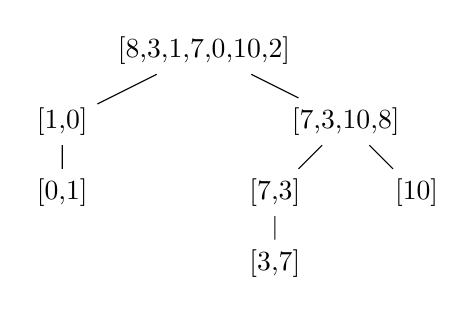
\begin{tikzpicture}[scale=0.6, level distance=1.5cm,
    level 1/.style={sibling distance=6cm},
    level 2/.style={sibling distance=3cm},
    level 3/.style={sibling distance=1.5cm}]

    \node {[8,3,1,7,0,10,2]}
      child {node {[1,0]}
        child {node {[0,1]}}
      }
      child {node {[7,3,10,8]}
        child {node {[7,3]}
          child {node {[3,7]}}
        }
        child {node {[10]}}
      };
  \end{tikzpicture}
  \end{center}

  \vspace{0.3cm}
  \textbf{Recursion Depth:}
  \begin{itemize}
    \item Best/Average case: $O(\log n)$
    \item Worst case (sorted input): $O(n)$
  \end{itemize}
\end{frame}

\begin{frame}[fragile]{Tail Recursion Optimization}
\begin{lstlisting}[language=Python, basicstyle=\ttfamily\tiny]
def quick_sort_tail_recursive(arr, low, high):
    """Optimize tail recursion to reduce stack space"""
    while low < high:
        pivot_idx = partition(arr, low, high)

        # Recurse on smaller partition
        if pivot_idx - low < high - pivot_idx:
            quick_sort_tail_recursive(arr, low, pivot_idx - 1)
            low = pivot_idx + 1
        else:
            quick_sort_tail_recursive(arr, pivot_idx + 1, high)
            high = pivot_idx - 1
\end{lstlisting}

\vspace{0.3cm}
\textbf{Benefit:}
\begin{itemize}
  \item Guarantees $O(\log n)$ stack depth
  \item Always recurse on smaller partition
  \item Convert tail call to iteration
\end{itemize}
\end{frame}

\begin{frame}[fragile]{Iterative Quick Sort}
\begin{lstlisting}[language=Python, basicstyle=\ttfamily\tiny]
def quick_sort_iterative(arr):
    """Quick sort without recursion"""
    stack = [(0, len(arr) - 1)]

    while stack:
        low, high = stack.pop()

        if low < high:
            pivot_idx = partition(arr, low, high)

            # Push subproblems to stack
            stack.append((low, pivot_idx - 1))
            stack.append((pivot_idx + 1, high))
\end{lstlisting}

\vspace{0.3cm}
\textbf{Advantages:}
\begin{itemize}
  \item No recursion overhead
  \item Explicit stack control
  \item Easier to debug
\end{itemize}
\end{frame}

\section{Time/Space Complexities}

\begin{frame}{Time Complexity: Comparison Sorts}
  \begin{center}
  \begin{tabular}{|l|c|c|c|}
    \hline
    \textbf{Algorithm} & \textbf{Best} & \textbf{Average} & \textbf{Worst} \\
    \hline
    Bubble Sort & $O(n)$ & $O(n^2)$ & $O(n^2)$ \\
    \hline
    Selection Sort & $O(n^2)$ & $O(n^2)$ & $O(n^2)$ \\
    \hline
    Insertion Sort & $O(n)$ & $O(n^2)$ & $O(n^2)$ \\
    \hline
    Merge Sort & $O(n \log n)$ & $O(n \log n)$ & $O(n \log n)$ \\
    \hline
    Quick Sort & $O(n \log n)$ & $O(n \log n)$ & $O(n^2)$ \\
    \hline
    Heap Sort & $O(n \log n)$ & $O(n \log n)$ & $O(n \log n)$ \\
    \hline
  \end{tabular}
  \end{center}

  \vspace{0.3cm}
  \textbf{Notes:}
  \begin{itemize}
    \item \textbf{Bubble/Insertion}: $O(n)$ best case when nearly sorted
    \item \textbf{Selection}: Always $O(n^2)$, even if sorted
    \item \textbf{Quick Sort}: Worst case with poor pivot selection
    \item \textbf{Merge/Heap}: Guaranteed $O(n \log n)$
  \end{itemize}
\end{frame}

\begin{frame}{Space Complexity}
  \begin{center}
  \begin{tabular}{|l|c|c|}
    \hline
    \textbf{Algorithm} & \textbf{Space} & \textbf{Type} \\
    \hline
    Bubble Sort & $O(1)$ & In-place \\
    \hline
    Selection Sort & $O(1)$ & In-place \\
    \hline
    Insertion Sort & $O(1)$ & In-place \\
    \hline
    Merge Sort & $O(n)$ & Not in-place \\
    \hline
    Quick Sort & $O(\log n)$ & In-place (stack) \\
    \hline
    Heap Sort & $O(1)$ & In-place \\
    \hline
    Counting Sort & $O(k)$ & Not in-place \\
    \hline
    Radix Sort & $O(n + k)$ & Not in-place \\
    \hline
  \end{tabular}
  \end{center}

  \vspace{0.3cm}
  \textbf{Key Points:}
  \begin{itemize}
    \item Stack space for recursion counts
    \item In-place sorts use $O(1)$ or $O(\log n)$
    \item Non-comparison sorts often require extra space
  \end{itemize}
\end{frame}

\begin{frame}{Lower Bound for Comparison Sorts}
  \textbf{Theorem}: Any comparison-based sort needs $\Omega(n \log n)$ comparisons

  \vspace{0.3cm}
  \textbf{Proof Idea:}
  \begin{itemize}
    \item Decision tree model: each comparison is a binary decision
    \item Tree must have at least $n!$ leaves (all possible permutations)
    \item Height of binary tree $\geq \log_2(n!)$
    \item Using Stirling's approximation: $\log_2(n!) \approx n \log_2 n$
  \end{itemize}

  \vspace{0.3cm}
  \textbf{Implications:}
  \begin{itemize}
    \item Merge Sort and Heap Sort are asymptotically optimal
    \item Quick Sort optimal in average case
    \item Cannot do better than $O(n \log n)$ with comparisons
    \item Non-comparison sorts can beat this bound!
  \end{itemize}
\end{frame}

\begin{frame}{Practical Performance Comparison}
  \textbf{Benchmark Results (n = 10,000):}

  \vspace{0.3cm}
  \begin{center}
  \begin{tabular}{|l|c|}
    \hline
    \textbf{Algorithm} & \textbf{Time (seconds)} \\
    \hline
    Quick Sort & 0.0120 \\
    \hline
    Merge Sort & 0.0180 \\
    \hline
    Heap Sort & 0.0250 \\
    \hline
    Timsort (Python) & 0.0015 \\
    \hline
    Insertion Sort & 1.2000 \\
    \hline
  \end{tabular}
  \end{center}

  \vspace{0.3cm}
  \textbf{Observations:}
  \begin{itemize}
    \item Quick Sort fastest among simple implementations
    \item Timsort (Python's built-in) highly optimized
    \item Insertion Sort impractical for large arrays
    \item Constants matter in practice!
  \end{itemize}
\end{frame}

\section{Non-Comparison Sorts: Counting/Radix}

\begin{frame}{Counting Sort: Overview}
  \textbf{Count Occurrences of Each Value}

  \vspace{0.3cm}
  \textbf{Algorithm:}
  \begin{enumerate}
    \item Count occurrences of each value
    \item Calculate cumulative counts
    \item Place elements in output array using counts
  \end{enumerate}

  \vspace{0.3cm}
  \textbf{Characteristics:}
  \begin{itemize}
    \item \textbf{Time}: $O(n + k)$ where $k$ = range of values
    \item \textbf{Space}: $O(k)$
    \item \textbf{Stable}: Yes
    \item \textbf{Limitation}: Only for integers in known range
  \end{itemize}

  \vspace{0.3cm}
  \textbf{When to Use:}
  \begin{itemize}
    \item Small range: $k \approx n$ or $k < n$
    \item Need linear time sorting
    \item Integers or can map to integers
  \end{itemize}
\end{frame}

\begin{frame}[fragile]{Counting Sort: Implementation}
\begin{lstlisting}[language=Python, basicstyle=\ttfamily\tiny]
def counting_sort(arr):
    """Sort array of non-negative integers"""
    if not arr:
        return arr

    # Find range
    max_val = max(arr)
    min_val = min(arr)
    range_size = max_val - min_val + 1

    # Count occurrences
    count = [0] * range_size
    for num in arr:
        count[num - min_val] += 1

    # Calculate cumulative count
    for i in range(1, range_size):
        count[i] += count[i - 1]

    # Build output array (stable)
    output = [0] * len(arr)
    for i in range(len(arr) - 1, -1, -1):
        num = arr[i]
        index = count[num - min_val] - 1
        output[index] = num
        count[num - min_val] -= 1

    return output
\end{lstlisting}
\end{frame}

\begin{frame}{Counting Sort: Example}
  \textbf{Sort: [4, 2, 2, 8, 3, 3, 1]}

  \vspace{0.3cm}
  \textbf{Step 1: Count occurrences}
  \begin{center}
  Count array (for values 1-8): [1, 2, 2, 1, 0, 0, 0, 1]

  Value: 1 appears 1x, 2 appears 2x, 3 appears 2x, etc.
  \end{center}

  \vspace{0.3cm}
  \textbf{Step 2: Cumulative count}
  \begin{center}
  [1, 3, 5, 6, 6, 6, 6, 7]
  \end{center}

  \vspace{0.3cm}
  \textbf{Step 3: Build output}
  \begin{center}
  Output: [1, 2, 2, 3, 3, 4, 8]
  \end{center}

  \vspace{0.3cm}
  \textbf{Time}: $O(n + k)$ where $n=7$, $k=8$
\end{frame}

\begin{frame}{Radix Sort: Overview}
  \textbf{Sort Digit by Digit Using Stable Sort}

  \vspace{0.3cm}
  \textbf{Algorithm (LSD - Least Significant Digit):}
  \begin{enumerate}
    \item Sort by least significant digit (using counting sort)
    \item Move to next digit
    \item Repeat until most significant digit
  \end{enumerate}

  \vspace{0.3cm}
  \textbf{Characteristics:}
  \begin{itemize}
    \item \textbf{Time}: $O(d(n + k))$ where $d$ = digits, $k$ = base
    \item \textbf{Space}: $O(n + k)$
    \item \textbf{Stable}: Yes
  \end{itemize}

  \vspace{0.3cm}
  \textbf{Applications:}
  \begin{itemize}
    \item Fixed-length integers or strings
    \item Card sorting machines (historical)
    \item Suffix array construction
  \end{itemize}
\end{frame}

\begin{frame}[fragile]{Radix Sort: Implementation}
\begin{lstlisting}[language=Python, basicstyle=\ttfamily\tiny]
def radix_sort(arr):
    """Sort array using radix sort (base 10)"""
    if not arr:
        return arr

    # Find maximum number to know number of digits
    max_num = max(arr)

    # Do counting sort for every digit
    exp = 1
    while max_num // exp > 0:
        counting_sort_by_digit(arr, exp)
        exp *= 10

def counting_sort_by_digit(arr, exp):
    """Counting sort by specific digit"""
    n = len(arr)
    output = [0] * n
    count = [0] * 10  # Base 10

    # Count occurrences of digits
    for num in arr:
        digit = (num // exp) % 10
        count[digit] += 1

    # Cumulative count
    for i in range(1, 10):
        count[i] += count[i - 1]

    # Build output (stable)
    for i in range(n - 1, -1, -1):
        digit = (arr[i] // exp) % 10
        output[count[digit] - 1] = arr[i]
        count[digit] -= 1

    # Copy to original array
    for i in range(n):
        arr[i] = output[i]
\end{lstlisting}
\end{frame}

\begin{frame}{Radix Sort: Example}
  \textbf{Sort: [170, 45, 75, 90, 802, 24, 2, 66]}

  \vspace{0.3cm}
  \textbf{Pass 1: Sort by 1's digit}
  \begin{center}
  [17{\color{red}0}, 9{\color{red}0}, 80{\color{red}2}, {\color{red}2}, 2{\color{red}4}, 4{\color{red}5}, 7{\color{red}5}, 6{\color{red}6}]

  Result: [170, 90, 802, 2, 24, 45, 75, 66]
  \end{center}

  \vspace{0.3cm}
  \textbf{Pass 2: Sort by 10's digit}
  \begin{center}
  [8{\color{red}0}2, {\color{red}0}2, 1{\color{red}7}0, {\color{red}2}4, {\color{red}4}5, 6{\color{red}6}, {\color{red}7}5, {\color{red}9}0]

  Result: [802, 2, 24, 45, 66, 170, 75, 90]
  \end{center}

  \vspace{0.3cm}
  \textbf{Pass 3: Sort by 100's digit}
  \begin{center}
  [{\color{red}0}02, {\color{red}0}24, {\color{red}0}45, {\color{red}0}66, {\color{red}0}75, {\color{red}0}90, {\color{red}1}70, {\color{red}8}02]

  Final: [2, 24, 45, 66, 75, 90, 170, 802]
  \end{center}
\end{frame}

\begin{frame}{Bucket Sort}
  \textbf{Distribute into Buckets, Sort Each}

  \vspace{0.3cm}
  \textbf{Algorithm:}
  \begin{enumerate}
    \item Create buckets for value ranges
    \item Distribute elements into buckets
    \item Sort each bucket individually
    \item Concatenate sorted buckets
  \end{enumerate}

  \vspace{0.3cm}
  \textbf{Characteristics:}
  \begin{itemize}
    \item \textbf{Time}: $O(n + k)$ average, $O(n^2)$ worst
    \item \textbf{Best for}: Uniformly distributed data
    \item \textbf{Poor for}: Skewed distributions
  \end{itemize}

  \vspace{0.3cm}
  \textbf{Example Use Case:}
  \begin{itemize}
    \item Sorting floating-point numbers in [0, 1)
    \item External sorting (disk-based)
  \end{itemize}
\end{frame}

\begin{frame}{Non-Comparison Sorts: Comparison}
  \begin{center}
  \begin{tabular}{|l|c|p{4cm}|}
    \hline
    \textbf{Algorithm} & \textbf{Time} & \textbf{Best Use Case} \\
    \hline
    Counting Sort & $O(n + k)$ & Small integer range \\
    \hline
    Radix Sort & $O(d(n + k))$ & Fixed-length integers/strings \\
    \hline
    Bucket Sort & $O(n + k)$ & Uniform distribution \\
    \hline
  \end{tabular}
  \end{center}

  \vspace{0.3cm}
  \textbf{Limitations:}
  \begin{itemize}
    \item \textbf{Counting}: Requires known integer range
    \item \textbf{Radix}: Not for arbitrary data types
    \item \textbf{Bucket}: Performance depends on distribution
  \end{itemize}

  \vspace{0.3cm}
  \textbf{Advantage:}
  \begin{itemize}
    \item Can achieve $O(n)$ time (beats comparison lower bound)
  \end{itemize}
\end{frame}

\section{Practical Considerations}

\begin{frame}{Python's Timsort}
  \textbf{Hybrid: Merge Sort + Insertion Sort}

  \vspace{0.3cm}
  \textbf{Used in:}
  \begin{itemize}
    \item Python's \texttt{sort()} and \texttt{sorted()}
    \item Java's \texttt{Arrays.sort()} for objects
  \end{itemize}

  \vspace{0.3cm}
  \textbf{Key Features:}
  \begin{itemize}
    \item \textbf{Time}: $O(n \log n)$ worst, $O(n)$ best
    \item \textbf{Stable}: Yes
    \item \textbf{Optimized for}: Real-world data with existing order
  \end{itemize}

  \vspace{0.3cm}
  \textbf{How it Works:}
  \begin{itemize}
    \item Detects "runs" (already sorted subsequences)
    \item Uses insertion sort for small runs ($< 64$ elements)
    \item Merges runs intelligently
    \item Exploits partially sorted data
  \end{itemize}
\end{frame}

\begin{frame}{When to Use Each Algorithm}
  \textbf{Small Arrays (n $<$ 50):}
  \begin{itemize}
    \item \textbf{Insertion Sort}: Simple, fast for small data
  \end{itemize}

  \vspace{0.2cm}
  \textbf{Nearly Sorted Data:}
  \begin{itemize}
    \item \textbf{Insertion Sort}: $O(n)$ when nearly sorted
    \item \textbf{Timsort}: Excellent for real-world data
  \end{itemize}

  \vspace{0.2cm}
  \textbf{Large Arrays:}
  \begin{itemize}
    \item \textbf{Quick Sort}: Fastest average case
    \item \textbf{Merge Sort}: Guaranteed $O(n \log n)$, stable
    \item \textbf{Heap Sort}: In-place, guaranteed $O(n \log n)$
  \end{itemize}

  \vspace{0.2cm}
  \textbf{Limited Memory:}
  \begin{itemize}
    \item \textbf{Heap Sort}: $O(1)$ extra space
    \item \textbf{Quick Sort}: $O(\log n)$ stack space
  \end{itemize}

  \vspace{0.2cm}
  \textbf{Need Stability:}
  \begin{itemize}
    \item \textbf{Merge Sort}, \textbf{Timsort}, or \textbf{Counting/Radix}
  \end{itemize}
\end{frame}

\begin{frame}{Optimization Techniques}
  \textbf{1. Hybrid Approaches:}
  \begin{itemize}
    \item Use Insertion Sort for small subarrays ($< 10$ elements)
    \item Combine Quick Sort with Insertion Sort
    \item Timsort: Merge Sort + Insertion Sort
  \end{itemize}

  \vspace{0.2cm}
  \textbf{2. Pivot Selection (Quick Sort):}
  \begin{itemize}
    \item \textbf{Random}: Avoid worst case
    \item \textbf{Median-of-three}: First, middle, last
    \item \textbf{Ninther}: Median of medians
  \end{itemize}

  \vspace{0.2cm}
  \textbf{3. Three-Way Partitioning:}
  \begin{itemize}
    \item Handle duplicates efficiently
    \item $O(n)$ when many equal elements
  \end{itemize}

  \vspace{0.2cm}
  \textbf{4. Tail Recursion Elimination:}
  \begin{itemize}
    \item Reduce stack space to $O(\log n)$
    \item Convert to iterative version
  \end{itemize}
\end{frame}

\begin{frame}{Common Mistakes}
  \textbf{1. Using Bubble Sort for Large Data:}
  \begin{itemize}
    \item {\color{red} BAD}: $O(n^2)$ always
    \item {\color{blue} GOOD}: Use Quick/Merge/Heap Sort
  \end{itemize}

  \vspace{0.2cm}
  \textbf{2. Not Considering Stability:}
  \begin{itemize}
    \item {\color{red} BAD}: Quick Sort breaks secondary sort
    \item {\color{blue} GOOD}: Use stable sort (Merge Sort, Timsort)
  \end{itemize}

  \vspace{0.2cm}
  \textbf{3. Ignoring Data Characteristics:}
  \begin{itemize}
    \item {\color{red} BAD}: Quick Sort on sorted data ($O(n^2)$)
    \item {\color{blue} GOOD}: Insertion Sort or Timsort ($O(n)$)
  \end{itemize}

  \vspace{0.2cm}
  \textbf{4. Wrong Algorithm for Data Type:}
  \begin{itemize}
    \item {\color{red} BAD}: Comparison sort for small integers
    \item {\color{blue} GOOD}: Counting Sort ($O(n)$)
  \end{itemize}
\end{frame}

\begin{frame}{Decision Tree for Choosing Sort}
  \begin{center}
  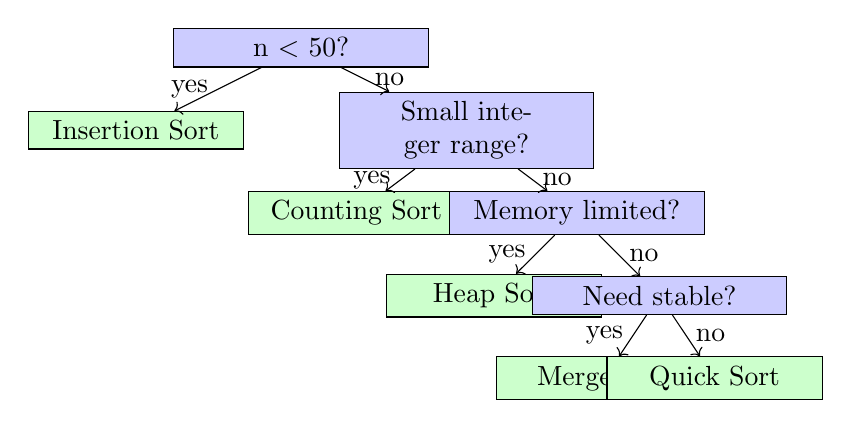
\begin{tikzpicture}[scale=0.7,
    decision/.style={rectangle, draw, fill=blue!20, text width=3cm, align=center},
    result/.style={rectangle, draw, fill=green!20, text width=2.5cm, align=center}]

    \node[decision] (start) at (0,0) {n $<$ 50?};
    \node[result] (ins) at (-3,-1.5) {Insertion Sort};
    \node[decision] (int) at (3,-1.5) {Small integer range?};
    \node[result] (count) at (1,-3) {Counting Sort};
    \node[decision] (mem) at (5,-3) {Memory limited?};
    \node[result] (heap) at (3.5,-4.5) {Heap Sort};
    \node[decision] (stable) at (6.5,-4.5) {Need stable?};
    \node[result] (merge) at (5.5,-6) {Merge Sort};
    \node[result] (quick) at (7.5,-6) {Quick Sort};

    \draw[->] (start) -- node[left] {yes} (ins);
    \draw[->] (start) -- node[right] {no} (int);
    \draw[->] (int) -- node[left] {yes} (count);
    \draw[->] (int) -- node[right] {no} (mem);
    \draw[->] (mem) -- node[left] {yes} (heap);
    \draw[->] (mem) -- node[right] {no} (stable);
    \draw[->] (stable) -- node[left] {yes} (merge);
    \draw[->] (stable) -- node[right] {no} (quick);
  \end{tikzpicture}
  \end{center}
\end{frame}

\section{Summary}

\begin{frame}{Key Takeaways}
  \textbf{Comparison Sorts:}
  \begin{itemize}
    \item \textbf{Quick Sort}: Fastest average case, in-place, unstable
    \item \textbf{Merge Sort}: Guaranteed $O(n \log n)$, stable, extra space
    \item \textbf{Heap Sort}: In-place, guaranteed $O(n \log n)$, unstable
  \end{itemize}

  \vspace{0.3cm}
  \textbf{Non-Comparison Sorts:}
  \begin{itemize}
    \item \textbf{Counting Sort}: $O(n + k)$, small integer range
    \item \textbf{Radix Sort}: $O(d(n + k))$, fixed-length data
    \item \textbf{Bucket Sort}: $O(n + k)$, uniform distribution
  \end{itemize}

  \vspace{0.3cm}
  \textbf{Important Properties:}
  \begin{itemize}
    \item \textbf{Stability}: Preserves relative order of equal elements
    \item \textbf{In-place}: Uses $O(1)$ or $O(\log n)$ extra space
    \item \textbf{Lower bound}: Comparison sorts need $\Omega(n \log n)$
  \end{itemize}
\end{frame}

\begin{frame}{Practical Recommendations}
  \textbf{For Most Cases:}
  \begin{itemize}
    \item Use language built-ins (e.g., Python's \texttt{sort()})
    \item They are highly optimized (Timsort, Introsort)
  \end{itemize}

  \vspace{0.3cm}
  \textbf{Implement Your Own When:}
  \begin{itemize}
    \item Learning algorithms
    \item Special requirements (stability, memory)
    \item Custom comparison logic
    \item Performance-critical applications
  \end{itemize}

  \vspace{0.3cm}
  \textbf{Quick Reference:}
  \begin{itemize}
    \item \textbf{General}: Quick Sort or Timsort
    \item \textbf{Guaranteed performance}: Merge Sort or Heap Sort
    \item \textbf{Small data}: Insertion Sort
    \item \textbf{Integer range}: Counting Sort or Radix Sort
    \item \textbf{Need stable}: Merge Sort or Timsort
  \end{itemize}
\end{frame}

\begin{frame}{Practice Problems}
  \textbf{Problem 1: Complexity Analysis}
  \begin{itemize}
    \item Why does Quick Sort have $O(n^2)$ worst case?
    \item How can we avoid it?
  \end{itemize}

  \vspace{0.2cm}
  \textbf{Problem 2: Algorithm Selection}
  \begin{itemize}
    \item Sort 1 million integers in range [0, 1000]
    \item Which algorithm is best? Why?
  \end{itemize}

  \vspace{0.2cm}
  \textbf{Problem 3: Stability}
  \begin{itemize}
    \item Sort students by grade, then by name
    \item Which sort preserves both orderings?
  \end{itemize}

  \vspace{0.2cm}
  \textbf{Problem 4: Implementation}
  \begin{itemize}
    \item Implement Quick Sort with median-of-three pivot
    \item Measure performance vs. last-element pivot
  \end{itemize}
\end{frame}

\begin{frame}{Resources}
  \textbf{Books:}
  \begin{itemize}
    \item "Introduction to Algorithms" (CLRS) - Chapter 6-9
    \item "The Algorithm Design Manual" (Skiena)
  \end{itemize}

  \vspace{0.3cm}
  \textbf{Online Visualizations:}
  \begin{itemize}
    \item VisuAlgo: visualgo.net/en/sorting
    \item Sorting Animations: sorting-algorithms.com
  \end{itemize}

  \vspace{0.3cm}
  \textbf{Practice:}
  \begin{itemize}
    \item LeetCode: Sort-related problems
    \item HackerRank: Sorting challenges
  \end{itemize}

  \vspace{0.3cm}
  \textbf{Advanced Topics:}
  \begin{itemize}
    \item Timsort implementation details
    \item Parallel sorting algorithms
    \item External sorting for big data
  \end{itemize}
\end{frame}

\end{document}
